\documentclass[18pt,a3paper,landscape, ncols=3]{cheatsheet}
\usepackage[style=boxed]{preamble}

% \usepackage{pdfpages} % included in `cheatsheet.sty`
\graphicspath{{graphics/}} % Sets the default location of pictures
% width=0.95\linewidth,totalheight=0.95\textheight,keepaspectratio
\setkeys{Gin}{keepaspectratio} % Improves figure scaling

% \begin{minipage}{0.5\textwidth}
% \end{minipage}%
% \begin{minipage}{0.5\textwidth}
% \end{minipage}

%%%%%%%%%%%%%%%%%%%%%%%%%%%%%%%%%%%%%%%%%%%%%%%%%%%%%%%%%%%%%%%%%%%%%%%%%%%%%%%
\begin{document}
%%%%%%%%%%%%%%%%%%%%%%%%%%%%%%%%%%%%%%%%%%%%%%%%%%%%%%%%%%%%%%%%%%%%%%%%%%%%%%%

% Foundations
\section{Statistics} \seperator
	\subsection{LLN}
		\begin{mdframed}
			\[
				\lim_{n \rightarrow \infinity} \abs{\frac{1}{n} \sum_{i=1}^{n} x_i - \Exp{x}} = 0
			\]
		\end{mdframed}
	\subsection{Unbiasedness}
		\begin{mdframed}
			\[
				\mathrm{Bias}_{\theta} = \Exp{\estimate{\theta}} - \theta = \Exp{\estimate{\theta} - \theta} = 0
			\]
		\end{mdframed}
	\subsection{Consistency}
		\begin{mdframed}
			\[
				\lim_{n \rightarrow \infinity} \Prob{ \abs{\widehat{X} - \frac{1}{n}\sum_{i=1}^{n} X_i} \leq \epsilon} = 1
			\]
		\end{mdframed}
	% \subsection{Hoeffding's Inequality}
	% 	\begin{mdframed}
	% 	\end{mdframed}
	% \subsection{Chebyshev's Inequality}
	% 	\begin{mdframed}
	% 	\end{mdframed}
	\subsection{Properties of Gaussians}
		\begin{mdframed}
			\[
				X \as \mathcal{N}(\mu,\, \sigma^2) \implies Y = aX + b \as \mathcal{N}(a\mu + b,\, a^2\sigma^2)
			\]
			\[
				X \as \mathcal{N}(\mu_x,\, \sigma^2_x),\,\qquad Y \as \mathcal{N}(\mu_y,\, \sigma^2_y),\,\quad \implies \quad Z = X + Y \as \mathcal{N}(\mu_x + \mu_y,\, \sigma^2_x + \sigma^2_y)
			\]
		\end{mdframed}
	% \subsection{Bayes Rule} % why not
	% 	\begin{mdframed}
	% 		% posterior, likelihood, prior, marginal
	% 		% unconditional version
	% 		% conditional version
	% 	\end{mdframed}
	% \subsection{Conjugate Prior}
	% 	\begin{mdframed}
	% 		% common conjugate priors...
	% 	\end{mdframed}

% % Foundations
% \section{Estimation} \seperator
% 	\subsection{MLE}
% 		\begin{mdframed}
% 		\end{mdframed}
% 	\subsection{MAP}
% 		\begin{mdframed}
% 		\end{mdframed}

% Foundations
\section{Information Theory} \seperator
	\subsection{Information \qquad\qquad\qquad\qquad\qquad\qquad Information Gain}
		\begin{mdframed}
			\begin{minipage}{0.5\linewidth}
				\[
					\Information{S} = \log_2 \frac{1}{\Prob{S}}
				\]
			\end{minipage}%
			\vrule%
			\begin{minipage}{0.5\linewidth}
				\[
					\Information{Y,\, X_i} = \Entropy{Y} - \Entropy{Y \given X_i}
				\]
			\end{minipage}
		\end{mdframed}
	\subsection{Entropy}
		\begin{mdframed}
			\begin{align*}
		    \Entropy{S} &= \sum_{s \in \Set{S}} \Prob{S{=}s} \cdot \Information{S{=}s} = \sum_{s \in \Set{S}} \Prob{S{=}s} \log_2 \frac{1}{\Prob{S{=}s}} \\
		                &=\quad\! \Exp{\log_2 \sfrac{1}{\Prob{S{=}s}}}\qquad\quad\, =\ {-} \Exp{\log_2 \Prob{S{=}s}} \\
		                &= {-} \sum_{s \in \Set{S}} \Prob{S{=}s} \log_2 \Prob{S{=}s}
		  \end{align*}
		\end{mdframed}

% Foundations
\section{Learning Theory} \seperator
	\subsection{PAC Learning}
		\begin{mdframed}
			\begin{minipage}{0.5\linewidth}%
				\[
					\Prob{\abs{\estimate{\theta} - \optimal{\theta}} \leq \epsilon} \geq 1 - \delta
				\]
			\end{minipage}%
			\vrule%
			\begin{minipage}{0.5\linewidth}%
				\[
					\Prob{\abs{\estimate{\theta} - \optimal{\theta}} > \epsilon} < \delta
				\]
			\end{minipage}
		\end{mdframed}

% Foundations
\section{Decision Theory} \seperator
	% \subsection{Common Loss Functions}
	% 	\begin{mdframed}
	% 	\end{mdframed}
	\subsection{Risk \qquad\qquad\qquad\qquad\qquad\qquad\qquad\qquad\quad Bayes Risk}
	\begin{mdframed}
		\begin{minipage}{0.5\linewidth}
			\[
				\mathrm{Risk}(f) = R(f) := \mathbb{E}_{(X,Y)} \Big[\loss \big(Y,\, f(X)\big)\Big]
			\]
		\end{minipage}%
		\qquad\vrule%
		\begin{minipage}{0.5\linewidth}
			\[
				R(f^*) \leq R(f),\ \forall\, f \in \mathcal{F}
			\]
		\end{minipage}
	\end{mdframed}
	\subsection{Bayes Optimal Rule}
		\begin{mdframed}
			\[
				f^{*}(P) = \argmin_{f} \mathbb{E}_{(X,Y) \as P} \Big[\loss \big(Y,\, f(X)\big)\Big]
			\]
		\end{mdframed}
	\subsection{Emperical Risk Minimization}
		\begin{mdframed}
			\[
				 \estimate{f}_{n} = \argmin_{f} \frac{1}{n} \sum_{i=1}^{n} \Big[\loss \big(Y_i,\, f(x_i)\big)\Big]\ \xrightarrow[n \rightarrow \infinity]{\quad\text{  LNN  }\quad}\ \argmin_{f} \mathbb{E}_{(X,\,Y)} \Big[\loss \big(Y,\, f(X)\big)\Big]
			\]
		\end{mdframed}

\columnbreak

% Foundations
\section{Risk} \seperator
	\subsection{True Risk \qquad\qquad\qquad\qquad\ Emperical Risk \qquad\qquad\quad Excess Risk}
		\begin{mdframed}
			\begin{minipage}{0.3\linewidth}
				\[
					R(f) := \mathbb{E}_{(X,Y)} \Big[\loss \big(f(X),\, Y\big)\Big]
				\]
			\end{minipage}%
			\hfill\vrule\hfill%
			\begin{minipage}{0.35\linewidth}
				\[
					\widehat{R}_{\mathcal{D}}(f) := \frac{1}{\Card{\mathcal{D}}} \sum_{i \in \mathcal{D}} \Big[\loss \big(f(X_i),\, Y_i\big)\Big]
				\]
			\end{minipage}%
			\hfill\vrule\hfill%
			\begin{minipage}{0.25\linewidth}
				\[
					\Exp{R(\estimate{f}_{n})} - R(\optimal{f})
				\]
			\end{minipage}
		\end{mdframed}
	\subsection{Structural Risk}
		\begin{mdframed}
			\begin{minipage}{0.35\linewidth}
				\begin{align*}
					& \abs{R(f) - \widehat{R}_{n}(f)} \leq C(f) & \forall\, f \in \mathcal{F} \\
					& R(f) \leq \widehat{R}_{n}(f) + C(f) & \forall\, f \in \mathcal{F}\\
				\end{align*}
				Use \(\widehat{R}_{n}(\estimate{f}_{n}) + C(\estimate{f}_{n})\) as a \textit{pessimistic} estimate of true risk.
			\end{minipage}%
			\begin{minipage}{0.65\linewidth}
				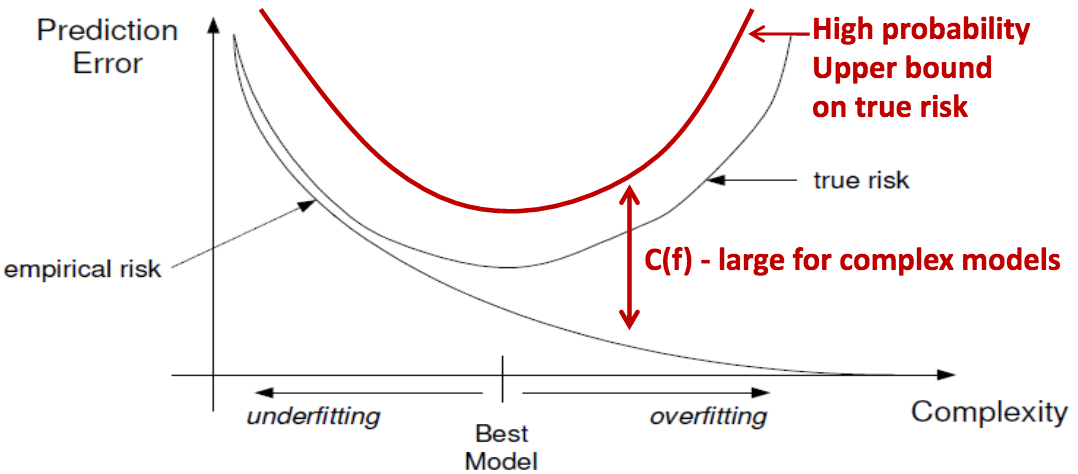
\includegraphics[width=\linewidth]{structural_risk_curve.png}
			\end{minipage}
		\end{mdframed}

	% Foundations
	\section{Risk Estimation}
		\subsection{Bias--Variance Tradeoff}
			\begin{mdframed}
				\begin{minipage}{0.3\linewidth}
					\begin{align*}
						\mathrm{Bias} &= \Exp{f(X)} - \optimal{f}(X) \\
						\mathrm{Variance} &= \Exp{{(f(X) - \Exp{f(X))}^2}} \\
						\mathrm{Bias}^2 &+ \mathrm{Variance} = \\
						& \Exp{{(f(X) - \optimal{f}(X))}^2}
					\end{align*}
				\end{minipage}%
				\hfill%
				\begin{minipage}{0.3\linewidth}
					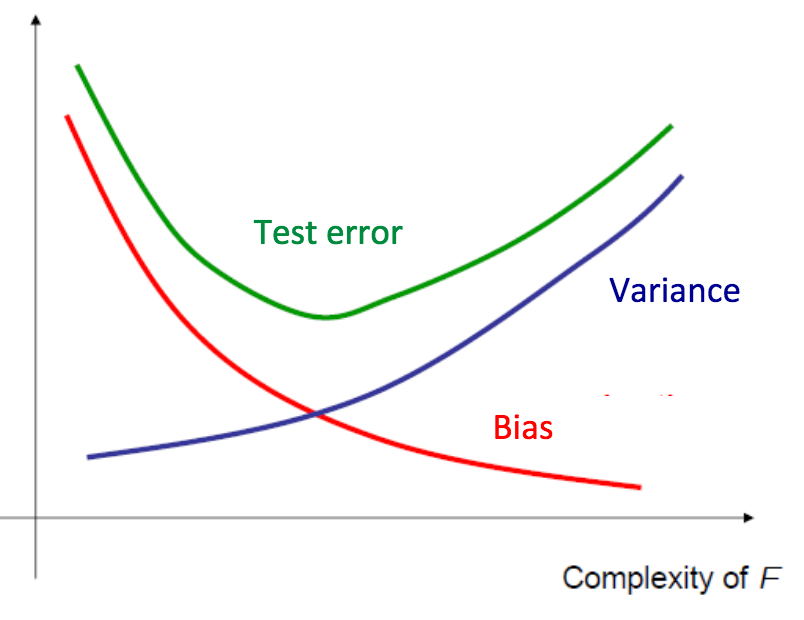
\includegraphics[width=\linewidth]{bias_vs_variance_error.png}
				\end{minipage}%
				\hfill%
				\begin{minipage}{0.3\linewidth}
					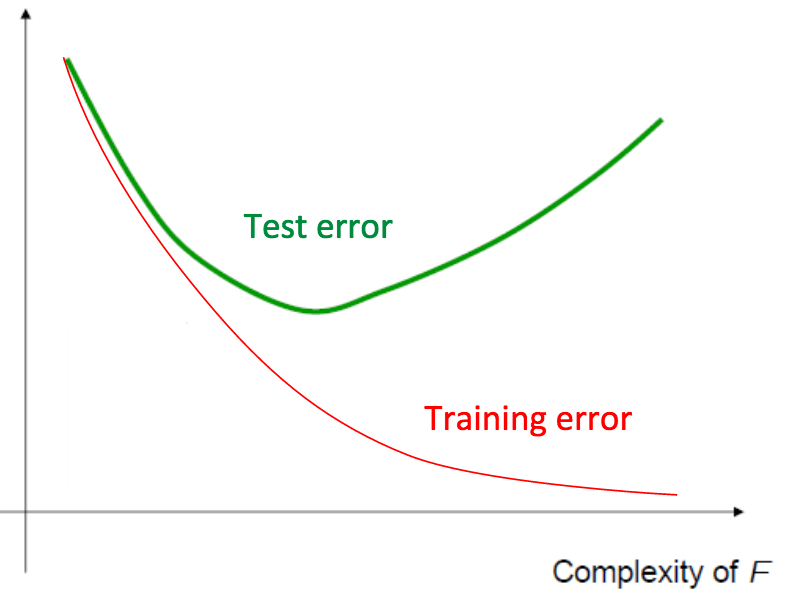
\includegraphics[width=\linewidth]{test_vs_train_error.png}
				\end{minipage}
			\end{mdframed}
		\subsection{K--Fold CV \qquad\qquad\qquad\quad LOO CV \qquad\qquad\qquad Random Subsampling}
			\begin{mdframed}
				% width=0.95\linewidth,totalheight=0.95\textheight,keepaspectratio
				\begin{minipage}{0.3\linewidth}
					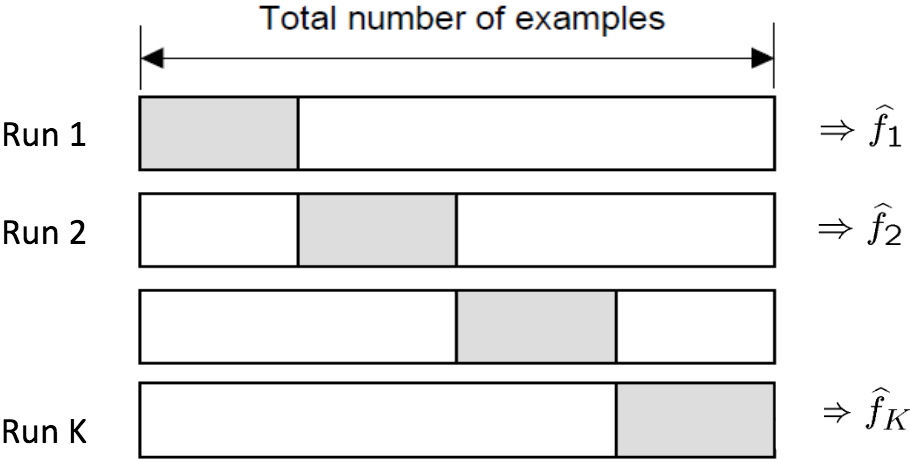
\includegraphics[width=\linewidth]{K_fold_cross_validation.png}
				\end{minipage}%
				\hfill%
				\begin{minipage}{0.3\linewidth}
					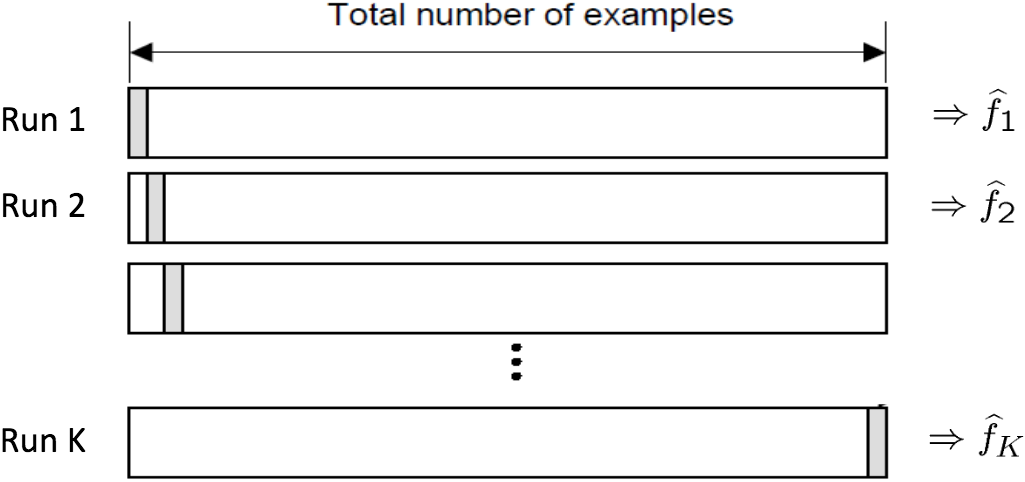
\includegraphics[width=\linewidth]{LOO_cross_validation.png}
				\end{minipage}%
				\hfill%
				\begin{minipage}{0.3\linewidth}
					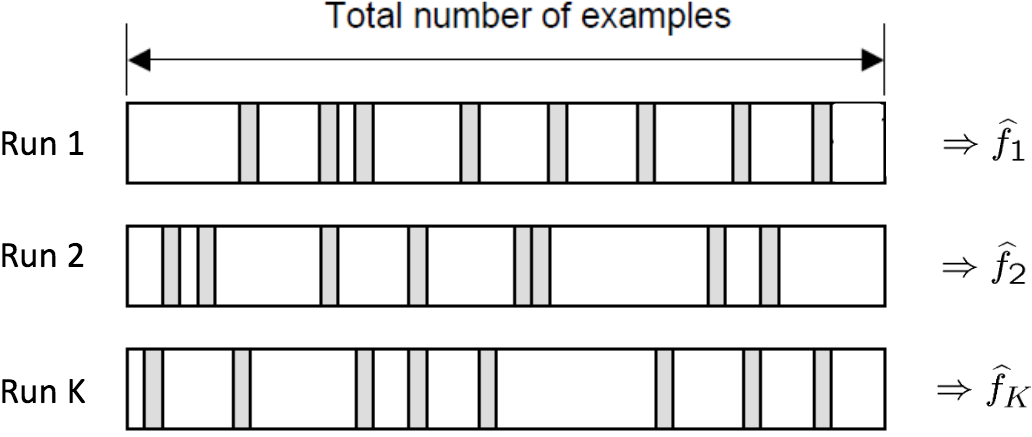
\includegraphics[width=\linewidth]{random_subsampling.png}
				\end{minipage}
			\end{mdframed}
		\subsection{Hold--out Method}
			\begin{mdframed}
				\begin{minipage}{0.4\linewidth}
					\begin{enumerate}[leftmargin=*]
						\item split into two sets
						\item use \(\mathcal{D}_{T}\) to train a predictor \(\estimate{f}_{\mathcal{D}_{T}}\)
						\item use \(\mathcal{D}_{V}\) to evaluate the predictor,
					\end{enumerate}
					\[
						\widehat{R}_{\mathcal{D}_{V}}(\estimate{f}_{\mathcal{D}_{T}})
					\]
				\end{minipage}%
				\hfill\vrule\hfill%
				\begin{minipage}{0.50\linewidth}
					\[
						\mathcal{D} = \Set{(X_i,\, Y_i)}_{i=1}^{n}
					\]
					\[
						\downarrow
					\]
					\[
						\underbrace{\mathcal{D}_{T} = \Set{(X_i,\, Y_i)}_{i=1}^{m}}_{\text{training set}}
						\qquad
						\underbrace{\mathcal{D}_{V} = \Set{(X_i,\, Y_i)}_{i=m+1}^{n}}_{\text{holdout set}}
					\]
				\end{minipage}
			\end{mdframed}
		\subsection{Estimating True Risk}
			\begin{mdframed}
				\begin{minipage}{0.5\linewidth}
					Estimate the error of a predictor on \(n\) data points.\\
					If K is large (close to \(n)\), bias of error estimate is small since each training set has close to \(n\) data points.\\
					However, variance of error estiamtes is high since each validation set has fewer data points and \(\widehat{R}_{V_{k}}\) might deviate a lot from the mean.\\
					\[
						\text{Error estimate} = \frac{1}{K} \sum_{k=1}^{K} \widehat{R}_{V_{k}} (\estimate{f}_{T_{k}})
					\]
				\end{minipage}%
				\begin{minipage}{0.5\linewidth}
					\hfill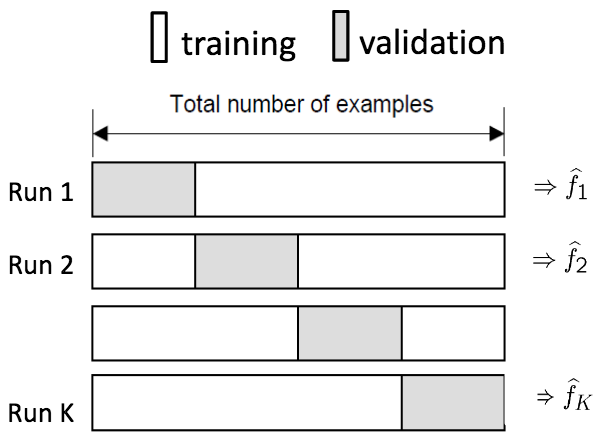
\includegraphics[width=0.85\linewidth]{estimating_true_risk.png}
				\end{minipage}
			\end{mdframed}

% Foundations
\section{Risk Minimization} \seperator
	\subsection{Emperical Risk Minimization \qquad\qquad\qquad Structural Risk Minimization}
		\begin{mdframed}
			\begin{minipage}{0.5\linewidth}
				\[
					\widehat{f_n} = \argmin_{f} \frac{1}{n} \sum_{i=1}^{n} \bigg[\loss \Big( Y_i,\, f(x_i) \Big) \bigg]
				\]
			\end{minipage}%
			\quad\vrule\quad%
			\begin{minipage}{0.5\linewidth}
				\[
					\estimate{f}_{n} = \argmin_{f \in \mathcal{F}} \Big\lbrack \widehat{R}_{n}(f) + \lambda C(f) \Big\rbrack
				\]
			\end{minipage}
		\end{mdframed}

\columnbreak

% Foundations
\section{Overfitting} \seperator
	\begin{mdframed}
		\begin{minipage}{0.3\linewidth}
			discrepency between emperical risk and true risk,\\ so emperical risk is no longer a good indicator of true risk
		\end{minipage}%
		\begin{minipage}{0.7\linewidth}
			\begin{center}
        \centering
        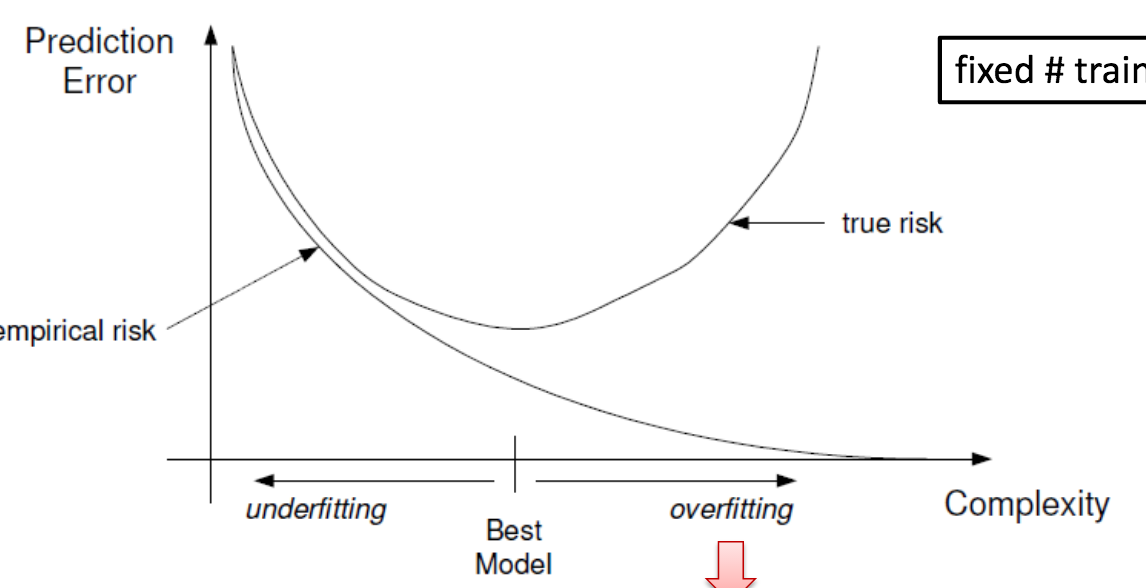
\includegraphics[width=\linewidth]{overfitting.png}
      \end{center}
		\end{minipage}
	\end{mdframed}

% Foundations
\section{Regularization} \seperator
	\subsection{Complexity Regularization}
		\begin{mdframed}
			\begin{minipage}{0.5\linewidth}%
				\[
					\estimate{f}_{n} = \argmin_{f \in \mathcal{F}} \Big\lbrace \widehat{R}_{n}(f) + \lambda C(f) \Big\rbrace
				\]
			\end{minipage}%
			\begin{minipage}{0.5\linewidth}%
				\begin{align*}
					C(f) &\ \colon\ \text{bound on deviation from true risk}\\
					\lambda &\ \colon\ \text{regularization penality}
				\end{align*}
			\end{minipage}
		\end{mdframed}
	\subsection{Information Criteria}
		\begin{mdframed}
			AIC (Akiake IC) \quad \(C(f) = \#\, parameters\)\\
			\indent Allows \(\#\) parameters to be infinite as \(\#\) training data \(n\) becomes large
		\end{mdframed}
		\begin{mdframed}
			BIC (Bayesian IC) \quad \(C(f) = \#\, parameters * \log n\)\\
			\indent Penalizes complex models more heavily -- limits complexity of models as \(\#\) training data \(n\) becomes large
		\end{mdframed}

% Foundations
\section{Model Selection} \seperator
	\begin{mdframed}
		\begin{itemize}
			\item define a finite set of model classes
			\item estimate true risk for each model class
			\item select model class with lowest estimated true risk
		\end{itemize}
	\end{mdframed}
	\begin{mdframed}
		Model classes \(\Set{\mathcal{F}_{\lambda}}\) of increasing complexity \(\mathcal{F}_{1} < \mathcal{F}_{2} < \ldots\)
		\[\min_{\lambda} \min_{f \in \mathcal{F}_{\lambda}} J(f,\, \lambda)\]
		\begin{itemize}
			\item given \(\lambda\) estimate \(\estimate{f}_{\lambda}\) using \textit{emperical / structural / complexity regularized} risk minimization
			\item select \(\lambda\) for which \(\estimate{f}_{\lambda}\) has minimum true risk estimated using \textit{cross--validation / hold--out / information criteria}
		\end{itemize}
	\end{mdframed}

% Foundations
\section{Generalization Error} \seperator
	\subsection{Terms}
		\begin{mdframed}
			\begin{minipage}{0.5\linewidth}
				\begin{gather*}
					\text{estimated predictor} := \estimate{f}_{n} \\
					\text{risk of estimated predictor} := R(\estimate{f}_{n}) \\
					\text{expected risk} := \Exp{R(\estimate{f}_{n})}
				\end{gather*}
			\end{minipage}%
			\begin{minipage}{0.5\linewidth}
				\begin{gather*}
					\text{optimal predictor} := \optimal{f} \\
					\text{risk of optimal predictor} := R(\optimal{f}) \\
					\text{excess risk} := \Exp{R(\estimate{f}_{n})} - R(\optimal{f})
				\end{gather*}
			\end{minipage}
		\end{mdframed}
	\subsection{True Risk Decomposition}
		\begin{mdframed}
		\[
			\Exp{R(\estimate{f}_{n})} - \optimal{R} = \underbrace{\Big\lparen \Exp{R(\estimate{f}_{n})} - \inf_{f \in \mathcal{F}} R(f) \Big\rparen}_{\text{estimation error}} + \underbrace{\Big\lparen \inf_{f \in \mathcal{F}} R(f) - \optimal{R} \Big\rparen}_{\text{approximation error}}
		\]
		\textit{Estimation Error} : due to randomness of training data \\
		\textit{Approximation Error} : due to restriction of model class \\
		\end{mdframed}
		\begin{mdframed}
			\begin{minipage}{0.5\linewidth}
				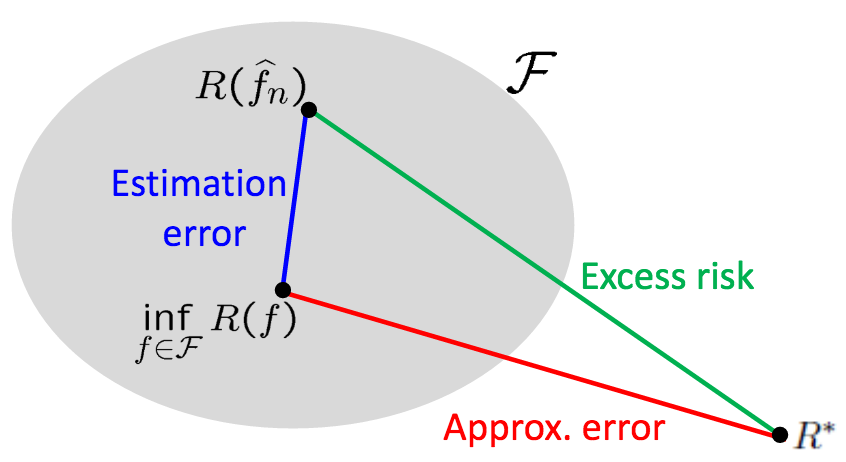
\includegraphics[width=0.95\linewidth]{true_risk_triangle.png}
			\end{minipage}%
			\begin{minipage}{0.5\linewidth}
				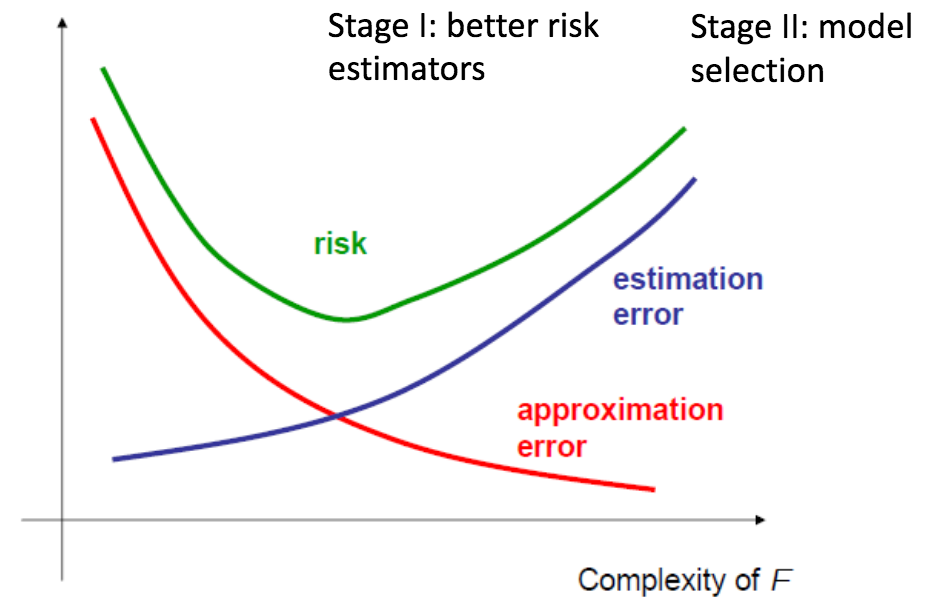
\includegraphics[width=0.5\linewidth]{true_risk_curve.png}
			\end{minipage}
		\end{mdframed}

\clearpage

% Parametric Models
\section{Regression} \seperator
	\subsection{Linear Regression}
		\begin{mdframed}
			\vspace{10mm}
		\end{mdframed}
		\begin{mdframed}
			\vspace{20mm}
		\end{mdframed}
	\subsection{Ridge Regression}
		\begin{mdframed}
			\[
				\estimate{\theta}_{\map}\argmin_{\theta} \sum_{i=1}^{n} {(Y_i - X_i \theta)}^2 + \lambda \norm{\theta}_{2}^{2}
			\]
		\end{mdframed}
		\begin{mdframed}
			\vspace{20mm}
		\end{mdframed}
	\subsection{Lasso Regression}
		\begin{mdframed}
			\[
				\estimate{\theta}_{\map}\argmin_{\theta} \sum_{i=1}^{n} {(Y_i - X_i \theta)}^2 + \lambda \norm{\theta}_{1}
			\]
		\end{mdframed}
		\begin{mdframed}
			\vspace{15mm}
		\end{mdframed}
	\subsection{Polynomial Regression}
		\begin{mdframed}
			\vspace{10mm}
		\end{mdframed}
		\begin{mdframed}
			\vspace{20mm}
		\end{mdframed}

% Parametric Models
\section{Classification} \seperator
	\subsection{Logistic Regression}
		\begin{mdframed}
			\vspace{10mm}
		\end{mdframed}
		\begin{mdframed}
			\vspace{20mm}
		\end{mdframed}
	\subsection{Naive Bayes}
		\begin{mdframed}
			\vspace{10mm}
		\end{mdframed}
		\begin{mdframed}
			\vspace{20mm}
		\end{mdframed}

\vfill\null
\columnbreak

	\subsection{Boosting}
		\begin{mdframed}
			\vspace{10mm}
		\end{mdframed}
		\begin{mdframed}
			\vspace{20mm}
		\end{mdframed}
	\subsection{Decision Trees}
		\begin{mdframed}
			\begin{align*}
		    \argmax_{X_i} \Big\lbrack \Entropy{Y} &- \Entropy{Y \given X_i} \Big\rbrack = \argmin_{X_i} \Entropy{Y \given X_i} \\
		      &= \argmin_{X_i} \sum_{x \in \Set{X_i}} \Big\lbrack \Prob{X_i{=}x} \Entropy{Y \given X_i{=}x} \Big\rbrack \\
		      &= \argmin_{X_i} {-} \sum_{x \in \Set{X_i}} \bigg\lbrack \Prob{X_i{=}x} \sum_{y \in \Set{Y}} \Big\lbrack \Prob{Y{=} \given X_i{=}x} \log_2 \Prob{Y{=}y \given X_i{=}x} \Big\rbrack \bigg\rbrack
		  \end{align*}
		\end{mdframed}
		\begin{mdframed}
			\vspace{20mm}
		\end{mdframed}
	\subsection{Support Vector Machines}
		\begin{mdframed}
			\vspace{10mm}
		\end{mdframed}
		\begin{mdframed}
			\vspace{30mm}
		\end{mdframed}

% Parametric Models
\section{Deep Learning} \seperator
	\subsection{Common Activation Functions}
		\begin{mdframed}
			\vspace{20mm}
		\end{mdframed}
	\subsection{Backpropagation}
		\begin{mdframed}
			\vspace{35mm}
		\end{mdframed}
	\subsection{Gradient Descent}
		\begin{mdframed}
			\vspace{35mm}
		\end{mdframed}
	\subsection{Perceptron}
		\begin{mdframed}
			\vspace{15mm}
		\end{mdframed}
	\subsection{MLP}
		\begin{mdframed}
			\vspace{15mm}
		\end{mdframed}
	\subsection{CNN}
		\begin{mdframed}
			\vspace{15mm}
		\end{mdframed}
	\subsection{RNN}
		\begin{mdframed}
			\vspace{15mm}
		\end{mdframed}
	\subsection{LSTM}
		\begin{mdframed}
			\vspace{15mm}
		\end{mdframed}

% Non--Parametric Models
\section{Clustering} \seperator % Supervised Learning
	\subsection{KNN}
		\begin{mdframed}
			\vspace{10mm}
		\end{mdframed}
		\begin{mdframed}
			\vspace{15mm}
		\end{mdframed}
	\subsection{Kernel Regression}
		\begin{mdframed}
			\vspace{10mm}
		\end{mdframed}
		\begin{mdframed}
			\vspace{15mm}
		\end{mdframed}
	\subsection{Kernel Trick}
		\begin{mdframed}
			\vspace{15mm}
		\end{mdframed}

%%%%%%%%%%%%%%%%%%%%%%%%%%%%%%%%%%%%%%%%%%%%%%%%%%%%%%%%%%%%%%%%%%%%%%%%
\end{document}
%%%%%%%%%%%%%%%%%%%%%%%%%%%%%%%%%%%%%%%%%%%%%%%%%%%%%%%%%%%%%%%%%%%%%%%%%%%%%%%%
